\newpage

\pgfplotsset{
  ylabel style={overlay},
  yticklabel style={overlay},
}

\definecolor{mycolor1}{rgb}{0.00000,0.44700,0.74100}%

\begin{figure}[H]
	\centering
    \begin{tikzpicture}
	\begin{axis}[%
        width=0.8\textwidth,
        height=0.6\textwidth,
        scale only axis,
        xmin=-90,
        xmax=90,
        xlabel style={font=\color{white!15!black}},
        xlabel={угол, град},
        ymin=-40,
        ymax=0,
        ylabel style={font=\color{white!15!black},yshift=10pt},
        ylabel={усиление, норм, дБ},
        ]
        \addplot [color=mycolor1, forget plot]  table [col sep=comma,x=theta, y=gain] {images/sect1-equally-spaced/equally-spaced-distribution-beam-pattern0.dat}; 
        
        % Add a node with a pin at coordinates (8.2, -13.2)
        \node[pin={[pin edge={thin}, pin distance=1ex]70:{$\theta=8.2, A=-13.2$}}] at (axis cs:8.2,-13.2) {};

        % Optional: Add a visible node marker
        \addplot [only marks, mark=*] coordinates {(8.2, -13.2)};
        
        % \node[pin={[pin edge={thin}, pin distance=1cm]290:{$\theta=8.2, A=-13.2$}}] at (8.2,-13.2) {};
        % \addplot [only marks] table {
        %     8.2 -13.2
        % };
    \end{axis}
    \end{tikzpicture}%
	\caption{ Диаграмма направленности рассчётной антенны}
	\label{fig:simulation-results}
\end{figure}


\begin{figure}[h]
    \centering
    \hspace*{-3ex}
    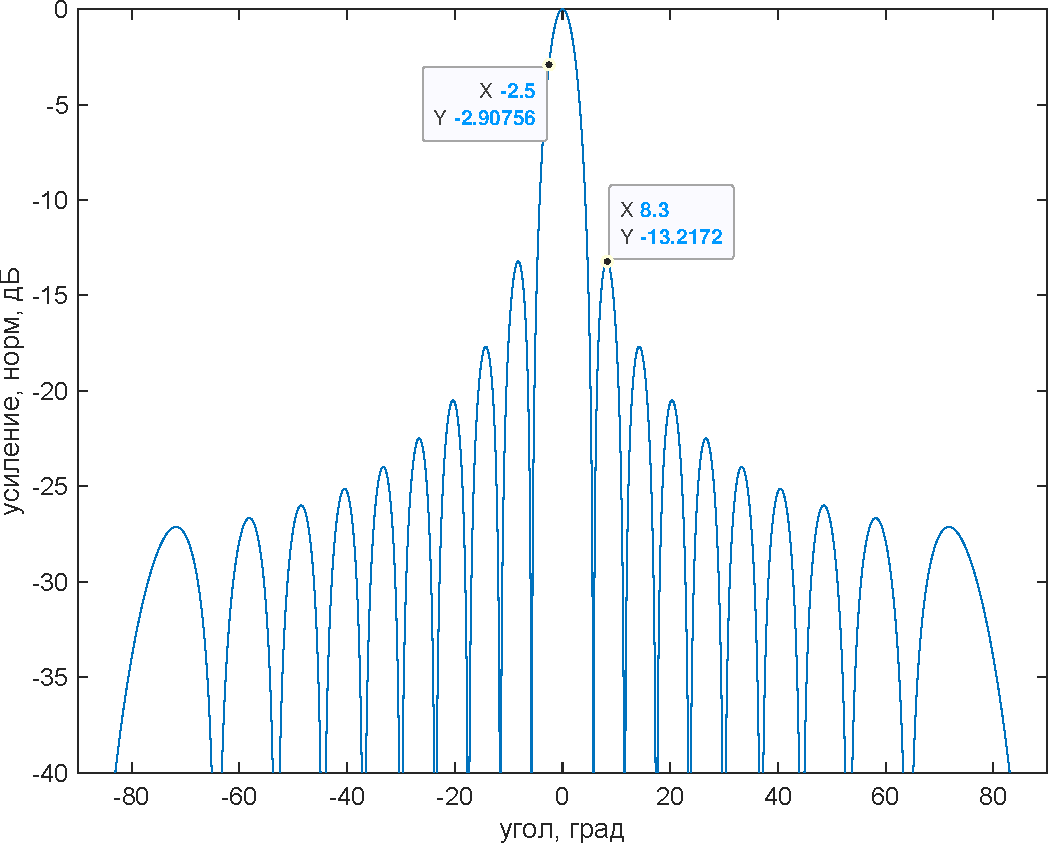
\includegraphics[width=0.8\textwidth]{equally-spaced-distribution-beam-pattern0}
	\caption{ Диаграмма направленности рассчётной антенны}
\end{figure}